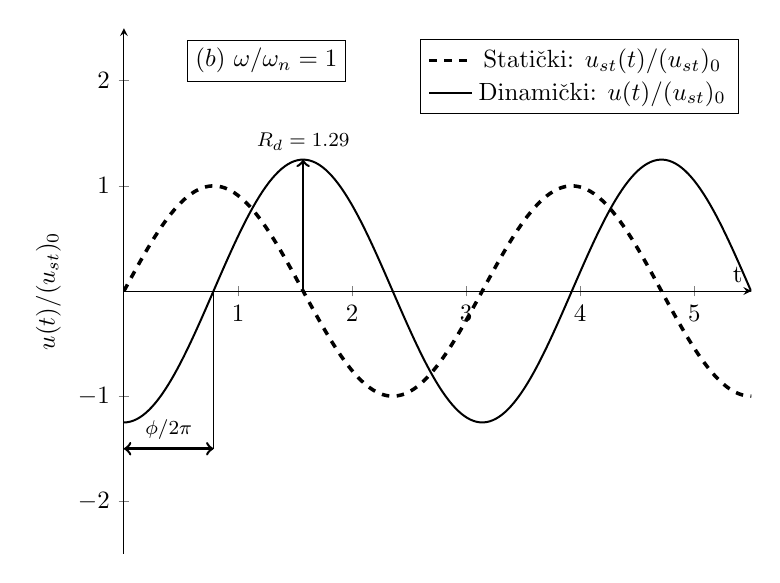
\begin{tikzpicture}[scale=0.9]
    \begin{axis} [
        title={$(b)\ \omega/\omega_n=1$},
        title style={at={(0.1,0.95)}, anchor=north west, draw=black, fill=white},
        height=9cm,
        axis lines = center,
        xlabel=t,ylabel=$u(t)/(u_{st})_0$,
        ylabel near ticks, ylabel style={anchor=south},
        xmin = 0, xmax = 5.5,
        ymin = -2.5, ymax = 2.5,
        xtick = {0, 1, 2, 3, 4, 5},
        ytick = {-2,-1, 0, 1, 2},
    ]
    \addplot [
        domain=0:5.5,
        samples=200,
        color=black,
        dashed, line width=0.5mm,
    ] {sin(2*deg(x))};
        \addlegendentry{Statički: $u_{st}(t)/(u_{st})_0$}
    \addplot [
        domain=0:5.5,
        samples=200,
        color=black,
        thick,
    ] {1.25*sin(2*deg(x)-90)};
        \addlegendentry{Dinamički: $u(t)/(u_{st})_0$}

        %kotiraj kut
        \draw ({pi*90/360},-1.5) -- ({pi*90/360},0);
        \draw[<->, line width=1pt] (0,-1.5) -- ({pi*90/360},-1.5)
            node[pos=0.5,above] {\footnotesize{$\phi/2\pi$}};

        %kotiraj dinamicki faktor
        \draw[->,line width=1pt] ({pi/4+pi*90/360},0) -- ({pi/4+pi*90/360},1.25)
            node[pos=1,above] {\footnotesize{$R_d=1.29$}};
    \end{axis}
\end{tikzpicture}
